%! Author = TiagoRG
%! GitHub = https://github.com/TiagoRG

\documentclass{report}
\usepackage[T1]{fontenc} % Fontes T1
\usepackage[utf8]{inputenc} % Input UTF8
\usepackage[backend=biber, style=ieee]{biblatex} % para usar bibliografia
\usepackage{csquotes}
\usepackage[portuguese]{babel} %Usar língua portuguesa
\usepackage{blindtext} % Gerar texto automaticamente
\usepackage[printonlyused]{acronym}
\usepackage{hyperref} % para autoref
\usepackage{graphicx}
\usepackage{indentfirst}
\usepackage{float}
\usepackage{geometry}

\geometry{
    paper=a4paper,
    margin=45pt,
    includefoot
}

\bibliography{bibliography}


\begin{document}
%%
% Definições
%! Author = TiagoRG
%! GitHub = https://github.com/TiagoRG

\newcommand{\titulo}{Mecânica e Campo Eletromagnético - Trabalho Prático 1}
\newcommand\data{DATA}
\newcommand\autores{Tiago Garcia, Rúben Gomes, Bruno Santos}
\newcommand\autorescontactos{(114184) tiago.rgarcia@ua.pt, (113435) rlcg@ua.pt, (113446) brunommsantos@ua.pt}
\newcommand\departamento{Dept. de Eletrónica, Telecomunicações e Informática}
\newcommand\empresa{Universidade de Aveiro}

%
%%%%%% CAPA %%%%%%
%
\begin{titlepage}

\begin{center}
%
\vspace*{50mm}
%
{\Huge \titulo}\\
%
\vspace{10mm}
%
{\Large \empresa}\\
%
\vspace{10mm}
%
{\LARGE \autores}\\
%
\vspace{30mm}
%
\begin{figure}[h]
\center

\includegraphics{images/ua}\label{fig:ua-title-logo}
\end{figure}
\end{center}
\end{titlepage}

%%  Página de Título %%
\title{%
{\Huge\textbf{\titulo}}\\
{\vspace{20mm}}
{\Large \departamento\\ \empresa}
}
%
\author{%
    \autores \\
    \autorescontactos
}
%
\date{\today}
%
\maketitle

%\pagenumbering{roman}



\tableofcontents
%\listoftables     % descomentar se necessário
%\listoffigures    % descomentar se necessário


%%%%%%%%%%%%%%%%%%%%%%%%%%%%%%%
\clearpage
\pagenumbering{arabic}


%%%%%% INTRODUÇÃO %%%%%%
%! Author = TiagoRG
%! GitHub = https://github.com/TiagoRG

\chapter{Introdução}
\label{ch:introducao}
{
%%%
% Conteúdo da introdução aqui
\section{Fórmulas} \label{sec:formulas}
    Para a resolução deste trabalho, foram consideradas as seguintes fórmulas, após certas deduções:
    \begin{itemize}
        \item $B_{sol} = \mu_0 (\frac{N}{l}) I_s$ (1)
        \item $\frac{\Delta C}{C} = \frac{\frac{\Delta N}{\Delta l}}{\frac{N}{l}} + \frac{\Delta m}{m}$ (2)
        \item $B = C_c V_H$ (3)
        \item $\vec{B}(x) = \frac{\mu_0 I R^2}{2(R^2 + (x - x_0)^2)^{3/2}}$ (4)
        \item $C_c = \frac{\mu_0 \frac{N}{l}}{m}$ (5)
        \item $\frac{N}{l} = \frac{B_{max}}{B_x}$ (6)
    \end{itemize}

    Para algumas destas fórmulas foi usada a constante $\mu_0$ que representa a permeabilidade magnética do vácuo, e é equivalente a $4\pi \times 10^{-7}~~Tm/A$.
%%%
\section{Objetivos} \label{sec:objetivos}
    O objetivo deste trabalho foi, na parte A, calibrar uma sonda de efeito de Hall, obtendo assim a sua constante de calibração ($C_c$), e calcular o seu respetivo erro.

    \par Na parte B, foi calculado o campo magnético ao longo do eixo de duas bobines na configuração de Helmholtz, utilizando uma sonda de Hall. \ Também foi estimado o número de espiras das bobines.
}



%%%%%%%%%%%%%%%%%%%%%%%%%%%%%%%%

% Capítulos
%! Author = TiagoRG
%! GitHub = https://github.com/TiagoRG

\chapter{Detalhes Experimentais Relevantes}
\label{ch:detalhes-experimentais-relevantes}
{
%%%
% Conteúdo da introdução aqui
\section{Material}
\label{subsec:detalhes-experimentais-relevantes-material}

\begin{enumerate}
    \item Voltímetro
    \item Amperímetro
    \item Fonte de tensão de $15~V$
    \item Resistência de $10~\Omega$
    \item Reóstato de $330~\Omega$
    \item Sonda de efeito de Hall
    \item Solenoide
    \item Bobines de Helmholtz
\end{enumerate}

\begin{figure}[H]
    \centering
    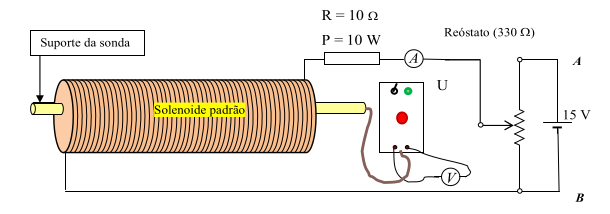
\includegraphics[width=1\linewidth]{images/esquema-montagem-experimental.png}
    \caption{Montagem experimental}
    \label{fig:detalhes-experimentais-relevantes-montagem-experimental}
\end{figure}

\pagebreak

\section{Parte A}
\label{sec:detalhes-experimentais-relevantes-parte1}

Esta primeira parte do trabalho foi realizada com o objetivo de calibrar a sonda de efeito de Hall, obtendo assim a sua constante de calibração ($C_c$), a ser usada na segunda parte do trabalho.

\subsection{Procedimento}
\label{subsec:detalhes-experimentais-relevantes-parte1-procedimento}

\begin{enumerate}
    \item Liga-se a sonda ao voltímetro e regula-se o potenciómetro da sonda para que o voltímetro indique $0~V$ quando não está sujeita a um campo magnético.
    \item Monta-se agora o resto do circuito, como na figura \ref{fig:detalhes-experimentais-relevantes-montagem-experimental}.
    \item Regista-se o valor $\frac{N}{l}$, que é o número de espiras por unidade de comprimento do solenoide.
    \item Coloca-se a sonda no interior do solenoide, procurando o ponto onde a aproximação utilizada de solenoide infinito.
    \item Ajusta-se o reóstato de modo a obter 10 valores de corrente $I_S$ diferentes, registando-se os diferentes valores da tensão $V_H$ para cada valor da corrente.
\end{enumerate}

\section{Parte B}
\label{sec:detalhes-experimentais-relevantes-parte2}

\subsection{Procedimento}
\label{subsec:detalhes-experimentais-relevantes-parte2-procedimento}

\begin{enumerate}
    \item Colocam-se as bobines na configuração de Helmholtz, com uma distância entre elas igual ao seu raio.
    \item Registam-se os dados das bobines, nomeadamente o raio e posição de cada uma.
    \item Monta-se agora o resto do circuito, como na figura \ref{fig:detalhes-experimentais-relevantes-montagem-experimental} apenas substituindo o solenoide por uma das bobines.
    \item Ajusta-se o reóstato de modo a ter $I=0.50A$ que será constante durante toda a experiência.
    \item Mede-se o campo magnético criado pela bobine ao longo do seu eixo, de centímetro a centímetro, registando cada par de valores: posição, tensão de Hall $(V_H)$.
    \item Repetem-se os passos 3, 4 e 5, mas agora para a segunda bobine (usando as mesmas posições usadas anteriormente).
    \item Ligam-se agora ambas as bobines, em série, e mais uma vez registam-se os valores da tensão de Hall para as mesmas posições utilizadas anteriormente.
\end{enumerate}

\pagebreak

%%%
}

%! Author = TiagoRG
%! GitHub = https://github.com/TiagoRG

\chapter{Análise e Discussão}
\label{ch:analise-discussao}
{
%%%
% Conteúdo da Análise e Discussão aqui

\section{Parte A}
\label{sec:analise-discussao-parte1}

\subsection{Análise}
\label{subsec:analise-discussao-parte1-analise}

\subsubsection{Distância}
\label{subsec:analise-discussao-parte1-distancia}

Esta distância é 10cm e será constante para todos os lançamentos sendo ela a distância entre os dois sensores de movimento. O erro associado a esta medição é de 1mm.

\subsubsection{Tempo}
\label{subsec:analise-discussao-parte1-tempo}

O tempo é medido pelo sistema de controlo dos sensores e é medido em segundo. O erro associado a esta medição é de 0.0001s. Este tempo é em média 0.04447s. A variação máxima do tempo é 0.0005s.

\subsubsection{Velocidade}
\label{subsec:analise-discussao-parte1-velocidade}

Para calcular a velocidade utilizamos a seguinte fórmula:

\begin{equation}
    v = \frac{d}{t}
\end{equation}

O erro associado a esta medição é de 0.0001m/s. A velocidade média é 2.249m/s. A variação máxima da velocidade é 0.04778m/s.

\subsection{Discussão}
\label{subsec:analise-discussao-parte1-discussao}

Tendo em conta as medições anteriores da distância e do tempo, verifica-se que a distância foi constante e a variação do tempo bastante baixa (variação máxima de 0.0005s) o que implica uma exatidão alta nos valores da velocidade calculados (exatidão de 97.9\%).\bigskip

Entre os possíveis motivos para a variação nos valores medidos de tempo podem se mencionar:
\begin{itemize}
    \item A falta de consistência da força da mola;
    \item A forma como a pessoa que dispara pode não o fazer exatamente da mesma forma em todos os disparos.
\end{itemize}

\pagebreak

\section{Parte B}
\label{sec:analise-discussao-parte2}

\subsection{Análise}
\label{subsec:analise-discussao-parte2-analise}

\subsubsection{Altura}
\label{subsec:analise-discussao-parte2-altura}

O valor da altura será constante e será medido desde o nível do alvo até ao ponto de lançamento verticalmente. No caso desta experiência, a altura medida foi 26cm.

\subsubsection{Ângulo}
\label{subsec:analise-discussao-parte2-angulo}

Este ângulo varia de lançamento para lançamento, sendo medido utilizando as marcações do lançador. O erro associado a esta medição é de 0.5º. Os valores usados foram 30º, 34º, 38º, 40º e 43º.

\subsubsection{Alcance}
\label{subsec:analise-discussao-parte2-alcance}

A figura \ref{fig:parte2-chart} representa o alcance em função do ângulo. No eixo $x$ temos o ângulo de lançamento enquanto que no eixo $y$ temos o alcance médio de cada ângulo.

\begin{figure}[ht]
    \centering
    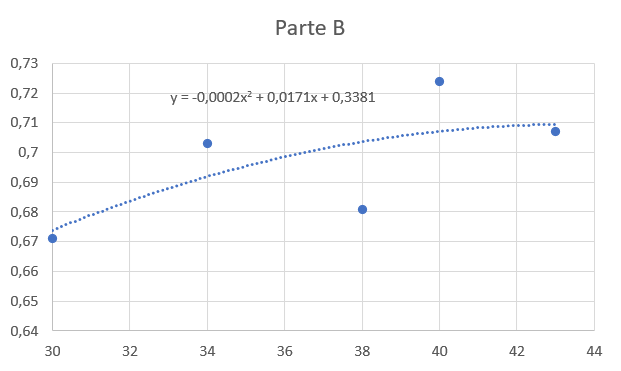
\includegraphics[width=0.6\textwidth]{images/parte2chart.png}
    \caption{Gráfico do alcance em função do ângulo}
    \label{fig:parte2-chart}
\end{figure}

\subsection{Discussão}
\label{subsec:analise-discussao-parte2-discussao}

Tendo em conta os valores obtidos, verifica-se uma maior discrepância entre esses mesmos valores, especialmente para os três primeiros ângulos usados (30º, 34º e 38º) com variações de 0.051, 0.046 e 0.046, respetivamente.\bigskip

Nesta experiência, estas variações podem se dever a diversos fatores, como por exemplo:
\begin{itemize}
    \item A falta de consistência da força da mola;
    \item A forma como a pessoa que dispara pode não o fazer exatamente da mesma forma em todos os disparos;
    \item A resistência do ar;
    \item As marcas existentes no alvo que podem causar confusão à pessoa que as vai verificar;
    \item A pouca estabilidade do alvo;
    \item Pequenas variações na forma de medição do alcance.
\end{itemize}\bigskip

Para calcular o ângulo para o qual o alcance é máximo, é necessário calcular a derivada da função do alcance em função do ângulo e igualar a zero. A função do alcance em função do ângulo foi obtida utilizando o software Microsoft Excel que aproximou uma função polinomial de segundo grau aos pontos respetivos aos nossos valores. A equação obtida foi, tal como se pode ver no gráfico da figura \ref{fig:parte2-chart}:

\begin{equation}
    y = -0.0002x^2 + 0.0171x + 0.3381
\end{equation}

A derivada desta função em $x$ será:

\begin{equation}
    y' = -0.0004x + 0.0171
\end{equation}\\
Por sua vez, esta será igual a 0 quando $x = 42.75$º.\bigskip

A altura de lançamento usada foi a mesma para todos os disparos de todos os ângulos o que implica que, baseado na experimentação, o ângulo para o qual se obtém maior alcance será $42.75$º.

\pagebreak

\section{Parte C}
\label{sec:analise-discussao-parte3}

\subsection{Análise}
\label{subsec:analise-discussao-parte3-analise}

\subsubsection{Comprimento do pêndulo}
\label{subsec:analise-discussao-parte3-comprimento}

Distância entre o ponto de suspensão e extremidade do centro. Este valor é obtido por medição direta com o erro associado de 1mm. O valor obtido foi de 24.4cm.

\subsubsection{Massas}
\label{subsec:analise-discussao-parte3-massas}

As massas são obtidas por medição direta com o erro associado de 0.1g. Os valores obtidos foram 237.2g para o pêndulo e 66.5g para o projétil.

\subsubsection{Ângulo}
\label{subsec:analise-discussao-parte3-angulo}

Este é o ângulo máximo descrito pelo movimento do pêndulo. O erro associado a esta medição é de 0.1º. O valor médio foi 17º.

\subsubsection{Altura}
\label{subsec:analise-discussao-parte3-altura}

Este é o valor da altura máxima atingida pelo projétil, que é registada no ponto de maior ângulo. Pode ser calculada a partir da seguinte fórmula:

\begin{equation}
    h = L(1 - \cos(\theta))
\end{equation}

O valor médio obtido foi 10.66mm.

\subsubsection{Velocidade}
\label{subsec:analise-discussao-parte3-velocidade}

Este é o valor da velocidade inicial do projétil. Pode ser calculada a partir da seguinte fórmula:

\begin{equation}
    v = \left| \frac{m_{projetil}~+~m_{pendulo}}{m_{projetil}} * \sqrt{2*g*h} \right|~~~~~(SI)
    \label{eq:parte3-velocidade-inicial}
\end{equation}

Onde $g$ é a aceleração gravítica e $h$ é a altura máxima atingida pelo projétil (calculada anteriormente).

\subsection{Discussão}
\label{subsec:analise-discussao-parte3-discussao}

Tendo em conta os valores obtidos, verifica-se uma amplitude de 1º. Esta variação pode se dever a diversos fatores, como por exemplo:

\begin{itemize}
    \item A falta de consistência da força da mola;
    \item A forma como a pessoa que dispara pode não o fazer exatamente da mesma forma em todos os disparos;
    \item Incerteza associada ao instrumento de medição;
    \item O atrito do pêndulo com o suporte.
\end{itemize}

Usando a fórmula \ref{eq:parte3-velocidade-inicial} obtém-se para cada ângulo diferentes valores de velocidade inicial, sendo o valor da velocidade média 2.0879m/s. Este resultado deverá ser semelhante ao obtido da Parte A (secção \ref{subsec:analise-discussao-parte1-velocidade}), que ao comparar verifica-se uma diferença de 0.1611m/s.

%%%
}


%%%%%% CONCLUSÕES %%%%%%
%! Author = TiagoRG
%! GitHub = https://github.com/TiagoRG

\chapter{Conclusões}
\label{ch:conclusoes}
{
%%%
% Conteúdo da conclusão aqui

Em todas as experiências, os objetivos essenciais foram cumpridos, contudo, verificámos alguns erros, como erros relacionados com medições que levaram a alguma disperidade entre valores calculados e valores teóricos.

De forma a reduzir/minimizar a variação do fator humano no disparo (ex. O lançamento ser efetuado sempre pela mesma pessoa), nas medições de forma a aumentar a precisão. Podem ser efetuadas mais medições com instrumentos mais rigorosos. Um exemplo disto é o alvo utilizado para medir o alcance na Parte B.

%%%
}


\pagebreak

\section*{$B_{sol} = \mu_0 \frac{N}{l} I_S$}
\begin{itemize}
    \item $B_{sol}$ - Campo magnético do solenóide (apenas paralelo ao eixo do solenóide)
    \item $\mu_0$ - Permeabilidade magnética do vácuo (constante, $4\pi \times 10^{-7}~~Tm/A$)
    \item $I_S$ - Corrente elétrica no solenóide
\end{itemize}

\section*{$\frac{\Delta C}{C} = \frac{\frac{\Delta N}{\Delta l}}{\frac{N}{l}} + \frac{\Delta m}{m}$}
Equação usada para calcular o erro relativo da constante de calibração do sensor de Hall.

\section*{$B = C_CV_V$}
Usada para calcular o campo magnético a partir da tensão de saída do sensor de Hall para as bobinas de Helmholtz.
\begin{itemize}
    \item $B$ - Campo magnético
    \item $C_C$ - Constante de calibração do sensor de Hall
    \item $V_V$ - Tensão de saída do sensor de Hall
\end{itemize}

\section*{$\vec{B}(x) = \frac{\mu_0 I R^2}{2(R^2 + (x - x_0)^2)^{3/2}}$}
As variáveis $x$ e $x_0$ anulam-se.
\begin{itemize}
    \item $\vec{B}(x)$ - Campo magnético no ponto $x$ do eixo do solenóide
    \item $\mu_0$ - Permeabilidade magnética do vácuo (constante, $4\pi \times 10^{-7}~~Tm/A$)
    \item $I$ - Corrente elétrica no solenóide
    \item $R$ - Raio do solenóide
\end{itemize}

\section*{$C_C = \frac{\mu_0 \frac{N}{l}}{m}$}
Resolve parte 1
\begin{itemize}
    \item $C_C$ - Constante de calibração do sensor de Hall
    \item $\mu_0$ - Permeabilidade magnética do vácuo (constante, $4\pi \times 10^{-7}~~Tm/A$)
    \item $m$ - Declive do gráfico $V_V = f(I_S)$
\end{itemize}

\section*{$\frac{N}{l} = \frac{B_{max}}{B_x}$}
Usada para calcular o número de espiras (parte 2)

%%%%%% ACRÓNIMOS %%%%%%
%%! Author = TiagoRG
%! GitHub = https://github.com/TiagoRG

\chapter*{Acrónimos}
\begin{acronym}
    \acro{deti}[DETI]{Departamento de Eletrónica, Telecomunicações e Informática}
    \acro{leci}[LECI]{Licenciatura em Engenharia de Computadores e Informática}
    \acro{ua}[UA]{Universidade de Aveiro}
\end{acronym}



%%%%%%%%%%%%%%%%%%%%%%%%%%%%%%%%%

\end{document}
